\documentclass[11pt,a4paper]{report}
\usepackage{ifpdf}
\usepackage[utf8]{inputenc}
\usepackage[francais]{babel}
\usepackage[french]{varioref} 
\usepackage[pdftex]{graphicx}
\usepackage{listings}
\usepackage{color}
\usepackage{amssymb}
\usepackage{amsmath}

%\usepackage{floatflt}
\usepackage{lscape} %afficher une partie en paysage


%%% Pour du code source %%%%
 \definecolor{colKeys}{rgb}{0.5,0,0.33} 
 \definecolor{colIdentifier}{rgb}{0.16,0,1} 
 \definecolor{colComments}{rgb}{0.25,0.5,0.37} 
 \definecolor{colString}{rgb}{0.6,0.1,0.1} 
 \definecolor{shadow}{rgb}{0.5,0.5,0.5} 
 
 \lstset{ 
 basicstyle=\ttfamily\small,
 identifierstyle=\color{colIdentifier},
 keywordstyle=\color{colKeys},
 stringstyle=\color{colString},
 commentstyle=\color{colComments}
 }
 \lstset{language=python}



\begin{document}

%1
\thispagestyle{empty}
\begin{center}
\begin{tabular}{lr}
\begin{minipage}[l]{0.4\textwidth}
\begin{flushleft}

\includegraphics[scale=0.2]{logo.png}
\end{flushleft}
\end{minipage}
&
\begin{minipage}[r]{0.4\textwidth}
\begin{flushright}
\begin{tabular}{l}
Van De Walle Bernard  (A)\\
Francois Thibault (B) \\
Van Der Essen Frédéric (C)
\end{tabular}
\end{flushright}
\end{minipage}
\end{tabular}
\end{center}

\vspace{6.5cm}

\begin{center}
\textsc{INGI2132: Langages et traducteurs}
\end{center}

\bigskip

\begin{center}
{\Huge Rapport Final}
\end{center}

\vspace{7.5cm}
\begin{center}
		\textbf{Prof.} B. Le Charlier\\
\end{center}

\vspace{1.5cm}

\newpage

\begin{figure}[h!]
\begin{center}
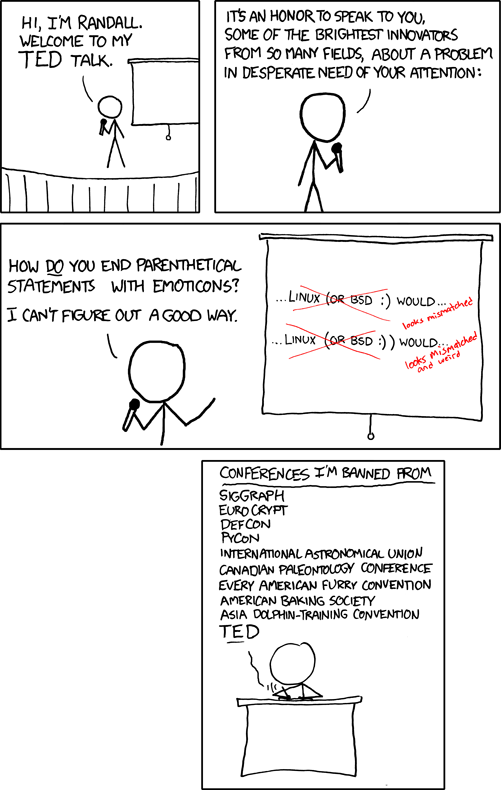
\includegraphics[scale=0.65]{xkcd.png}
\end{center}
\end{figure}
It is now possible with the HAPPY-) programming language !
\newpage

\tableofcontents
%2
\chapter*{Introduction}
	Voici le rapport final de notre projet où il nous était demandé de
	réaliser un interpréteur avec comme contrainte l'utilisation d'une
	syntaxe WP. 

	Nous pensons avoir complété l'entièreté du projet. Il reste cependant
	un oubli au niveau du vérificateur de grammaire : Celui ci ne vérifie
	pas la présence de Symboles non terminaux intermédiaires inutiles. 

	Le rapport suit à la lettre le plan donné dans les consignes. 


%3
\chapter{Présentation de Happy:-)}
\section{Introduction}
La langage happy, appelé ainsi parce qu'il est très permissif au niveau des caractères permit dans les identifiants comporte de nombreuses autres particularités. Tout d'abord, le langage ressemble très fort au LISP où tout est atom ou liste.
Mais contrairement au LISP, notre langage est impératif et orienté objet. Un programme est une liste de méthode, une méthode est une liste dont le premier élément est le mot réservé fun le second une list d'argument et le dernier une liste de commande. Même principe pour le while et le if. Dans ce langage tout est fonction, dans le sens que toute instruction renvoie une valeur, y compris les if et le while qui renvoient 0, une fonction qui n'a pas d'instruction return renvoie null, le write renvoie la valeur qu'elle vient d'imprimer etc...



Les conditions aurait aussi renvoyé une valeur si le langage SLIP dans lequel notre langage est traduit le permettait. 

\section{Grammaire de départ}
Cette grammaire est la grammaire exhaustive du langage si on rajoute que les id peuvent être formé de tout les caractères UTF-16 sauf des caractères réservés et qu'ils ne doivent pas être égale à un mot réservé.

\begin{verbatim}
<Program> ::= ( <Prog_list> )
<Prog_list> ::=  <Meth_or_fun> | <Prog_list> <Meth_or_fun>	
<Meth_or_fun> ::=  <Method> | <Function>

<Function> := ( fun ( <Arglist> ) <Instr_list> ) 
<Arglist> ::=  id | id <Arglist>
<Method> ::= ( <Method_int> ( <Arglist> ) <Instr_list> )
 
<Instr_list> ::=  <Instr> | ( <Instr_list_np> ) 
<Instr_list_np> ::=  <Instr> | <Instr> <Instr_list_np>
<Instr> ::=  <Conditional> | <While_block> | <Call> | ( return <Expr> ) 

<Conditional> ::= ( if <Cond> <instr_list> <instr_list>  )  
<Conditional> ::= ( if <Cond> <instr_list> )
<While_block> ::= ( while  <Cond> <Instr_list>  ) 
<call> ::=  <User_call> | <Method_call> | <Builtin_call> 
<Builtin_call> ::=  <Assignment> | <Read_call> | <Write_call> | <Arithmetic_call>
<Assignment> ::= ( set id <Expr> ) 
<Assignment> ::= ( set <Id_int> <Expr> ) | ( set <This_int> <Expr> )
<Read_call>  ::= ( read )
<Write_call> ::= ( write <Expr> )
<Arithmetic_call> ::=  <Binary> | <Unary>
<Binary> ::= ( <Bin_id> <Expr> <Expr>  )
<Unary>  ::= ( <Un_id> <Expr>  )
<User_call>  ::= ( id  <Expr_list_np> ) | ( id ) 
<Expr_list_np> ::=  <Expr> | <Expr> <Expr_list_np>
<Method_call>  ::= ( <Id_id> <Expr_list_np>  ) |  ( <Id_id> )   
<Method_call>  ::= ( <Super_id>  <Expr_list_np>  ) | ( <Super_id>  )
<Method_call>  ::= ( <This_id>  <Expr_list_np>  ) | ( <This_id> )
<Expr> ::= number | null | true | false | this | id 
<Expr> ::= <Id_int> | <This_int> | <Instr>
<Cond> ::= <Rel> | ( <Log_bin_op> <Cond> <Cond> )
<Cond> ::= ( <Log_un_op> <Cond> <Cond> )
<Rel>  ::= ( <Rel_op> <Expr> <Expr> ) 
<Rel_op> ::= <= | >= | > |  < | =
<Log_bin_op> ::= and | or
<Log_un_op> ::= !
<Bin_id> ::= + | - | * | / | %
<Un_id> ::= neg
<Id_int> ::= id . number
<This_int> ::= this . number
<Super_id> ::= super . id
<This_id> := this . id 
<Id_id> ::= id . id
<Method_int> ::= method . number
\end{verbatim}
Cette grammaire n'est pas wp, mais elle exprime très bien ce qui est syntaxiquement correcte dans ce que nous avons réellement implémenté. 

Voici quelque bout de code permis par cette grammaire :

\begin{verbatim}
[Le while s'écrit comme ceci while (la condition) (les instruction a répèter)
  ici la condition est 3 * i <= 9
On remarque aussi que sur ce bout de code on peut écrire 
la valeur de retour de set qui sera ici i_initial + 1 ou i_final ]
(while (<= (* 3  i) 9) (write (set i (+ i 1)))) 
  
[Condition ici si i != 9 ]
[Ensuite si vrai on exécute la première list d'instruction sinon la seconde]
(if (! (= i 9)) (return true) (return false))
[Ceci est équivalent à sauf que dans le cas deux on voit clairement les listes d'instructions]
(if (! (= i 9)) ((return true)) ((return false)))

(fun (++ i) (return (+ i 1)))

(set i (++ i))

(set a (new 2))
\end{verbatim}

\section{Exemple de programme complet}
Le premier programme imprime juste l'entier lu à la console.

\begin{verbatim}
(
  (fun (main) 
    (write (read))
  )
)
\end{verbatim}

Le programme suivant fait la somme de 1 à n pour 10 n
\begin{verbatim}
(
  [Programme fait la somme de 1 à n pour n qui va de 0 à 10]
  (fun (main) (
    (set i 0)
    (while (<= i 10)
    (
      (write (sum i))
      (set i (+ i 1))
    ))
  ))


  (fun (sum n) (
    (if (= n 0)
      (return 0)
    )
    (return (+ n (sum (- n 1))))
  ))
)

\end{verbatim}



Le dernier programme fait la somme des éléments d'une pile et utilise la POO
\begin{verbatim}
(
  (fun (main) (
    (set s ( >> 4 ( >> 3 (>> 2 (# 1)))))
    (write (s.@))
    (write (s.->))
    (set s (>> 5 s))
    (Print s)
    (write (sum s))
  ))
  [crée une nouvelle pile avec a comme élément au sommet]
  (fun (# a) (
    (set b (new 2))
    (b.@= a)
    (b.->= null)
    (return b)
  ))

  [Push sur la stack]
  [a : l'élément à mettre sur la stack]
  [s : la stack]
  (fun (>> a s) (
    (set n (new 2))
    (n.->= s)
    (n.@= a)
    (return n)
  )) 

  (fun (Print N) (
    (if (! (= N null)) (
      (write (N.@))
      (Print (N.->))
    )
    (write 0)
    )
  ))

  (fun (sum N) (
    (if (! (= N null)) 
      (return (+ (N.@) (sum (N.->))))
      (return 0)
    )
     
  ))
  [Accesseur pour l'élément contenu dans le noeud]
  (method.2 (@) (return this.1))
  ((method.2 (@= a) (set this.1 a))
  [Accesseur pour next]
  (method.2 (->) (return this.2))
  (method.2 (->= a) (set this.2 a))
)
\end{verbatim}




 
%4
\chapter{L'analyseur Lexical}

L'analyseur Lexical a pour fonction de sortir une suite de jetons concrets et de assez haut niveau, permettant de simplifier la tache du vérificateur de grammaire. Plus concrètement, il s'agit dans un premier temps de transformer un fichier texte en une suite de caractère, et de les parser les un après les autres. Chaque caractère donnera lieu à une action précise, par exemple les caractères spéciaux tel que les parenthèses et les points, etc... donnent lieux à un jeton entier.
Les caractères qui ne sont pas des caractères spéciaux vont quand à eux remplir un buffer , qui sera rempli des qu'un caractère spécial ou délimiteur sera rencontré. Une fois qu'un caractère de ce type est rencontré, on procédera à l'analyse de ce que contient le buffer, et selon le cas on en déterminera le type du jeton à donner.

\section{Entrée de l'analyseur lexical}

Il est important de préciser correctement ce que l'analyseur lexical doit prendre en entrée. Par soucis de facilité, nous avons décidé de nous restreindre aux caractères ascii 8 bits, et plus particulièrement, toutes les lettres ( miniscule et majuscule ), les chiffres, les opérateurs *,+,/-, le symbole d'égalité, les parenthèses, les crochets ( [] ) ,  et le point.

Ensuite il est nécessaire de définir les différents symboles de base que l'analyseur lexical va passer à l'analyseur syntaxique.

Voici donc les différentes catégories que l'analyseur lexical va sortir :

\begin{itemize}

\item NUMBER  : Représente un ou plusieurs chiffres à la suite.
\item ID : Représente une suite de caractères qui n'est pas un mot réservé.
\item $UNARY\_OP$ : Représente un opérateur unaire, tel que l'opérateur NOT : !
\item $BINARY\_OP$ : représente un opérateur binaire, tel l'opérateur +
\item $*RESERVED\_WORD*$: représente un mot réservé. En fait la catégorie sera le nom du mot réservé (d'où les étoiles ), par exemple FUN
\item $*BEFORE\_AFTER*$ : Représente ce qu'il y a avant et après un point. BEFORE et AFTER peuvent valoir : THIS, ID, INT

\end{itemize}



Finalement, il est de bon aloi de préciser que les espaces, les caractères de tabulations et de nouvelle ligne servent évidemment de caractère de séparation. Il n'est par contre pas nécessaire de placer un espace après une parenthèse par exemple, vu qu'il est assez naturel que ce qui suit sera le début d'un nouveau symbole.

Pour ce qui est des commentaires, nous avons introduit les symboles de crochet ( [] ). Tout ce qui se trouvera entre ces deux crochets ( et les crochets eux-même compris ), sera purement et simplement ignoré. Les commentaires peuvent donc s'étendre sur plusieurs lignes sans aucun problème.

Notre analyseur lexical ne renvoie plus de jetons à partir du moment où on atteind la fin du fichier. Il n'est pas nécessaire de terminer le fichier d'une manière particulière.


\section{Symboles terminaux de bases}
\begin{verbatim}
( ) <= >= > < = and or ! + - * / % neg id . number this super while 
if set write read fun method null true false 
 
\end{verbatim}
C'est-à-dire tout les mots réservé qui se trouve dans le tableau $RESERVED\_WORD$ dans la classe \textit{WordIdentifier.java} et tout le reste qui sont



\section{Grammaire formelle}
{\small
\begin{verbatim}
<Program> ::= ( <Prog_list> )
<Prog_list> ::=  <Meth_or_fun> | <Prog_list> <Meth_or_fun>	
<Meth_or_fun> ::=  <Method> | <Function>

<Function> := ( fun ( <Arglist> ) <Instr_list> ) 
<Arglist> ::=  id | id <Arglist>
<Method> ::= ( <Method_int> ( <Arglist> ) <Instr_list> )
 
<Instr_list> ::=  <Instr> | ( <Instr_list_np> ) 
<Instr_list_np> ::=  <Instr> | <Instr> <Instr_list_np>
<Instr> ::=  <Conditional> | <While_block> | <Call> | ( return <Expr> ) 

<Conditional> ::= ( if <Cond> <instr_list> <instr_list>  )  
<Conditional> ::= ( if <Cond> <instr_list> )
<While_block> ::= ( while  <Cond> <Instr_list>  ) 
<call> ::=  <User_call> | <Method_call> | <Builtin_call> 
<Builtin_call> ::=  <Assignment> | <Read_call> | <Write_call> | <Arithmetic_call>
<Assignment> ::= ( set id <Expr> ) 
<Assignment> ::= ( set <Id_int> <Expr> ) | ( set <This_int> <Expr> )
<Read_call>  ::= ( read )
<Write_call> ::= ( write <Expr> )
<Arithmetic_call> ::=  <Binary> | <Unary>
<Binary> ::= ( <Bin_id> <Expr> <Expr>  )
<Unary>  ::= ( <Un_id> <Expr>  )
<User_call>  ::= ( id  <Expr_list_np> ) | ( id ) 
<Expr_list_np> ::=  <Expr> | <Expr> <Expr_list_np>
<Method_call>  ::= ( <Id_id> <Expr_list_np>  ) |  ( <Id_id> )   
<Method_call>  ::= ( <Super_id>  <Expr_list_np>  ) | ( <Super_id>  )
<Method_call>  ::= ( <This_id>  <Expr_list_np>  ) | ( <This_id> )
<Expr> ::= number | null | true | false | this | id 
<Expr> ::= <Id_int> | <This_int> | <Instr>
<Cond> ::= <Rel> | ( <Log_bin_op> <Cond> <Cond> )
<Cond> ::= ( <Log_un_op> <Cond> <Cond> )
<Rel>  ::= ( <Rel_op> <Expr> <Expr> ) 
<Rel_op> ::= <= | >= | > |  < | =
<Log_bin_op> ::= and | or
<Log_un_op> ::= !
<Bin_id> ::= + | - | * | / | %
<Un_id> ::= neg
<Id_int> ::= id . number
<This_int> ::= this . number
<Super_id> ::= super . id
<This_id> := this . id 
<Id_id> ::= id . id
<Method_int> ::= method . number
\end{verbatim}}


\section{Représentation des symboles lexicaux}

Les Symboles lexicaux sont représenté à l'aide d'un objet de type LexicalTerm. Cet objet contient deux informations nécessaires. La première est la catégorie du symbole lexical, comme défini un peu plus haut. La seconde information est ce que contient concrètement le symbole lexical.
Afin de clarifier cela, un petit exemple s'impose : 
Imaginons que l'analyseur lexical découvre un identifiant pour le mot  "valeura" dans le fichier source. Dans ce cas, il créera un objet LexicalTerm contenant l'information suivante :
\begin{itemize}
\item TYPE : ID
\item CONTENT : valeura
\end{itemize}

Dans le cas où maintenant le mot réservé fun est rencontré, l'objet LexicalTerm alors créé contiendra : 
\begin{itemize}
\item TYPE : fun
\item CONTENT : fun
\end{itemize}

\section{Spécification rigoureuse des méthodes publiques de l'analyseur lexical}

De manière concrète, l'analyseur lexical a été réalisé en implémentant l'interface Iterator et Iterable. Les méthodes publiques seront dons les méthodes propres à ces interfaces . Les méthodes utilisées par l'analyseur syntaxique sont donc :

La méthode hasNext()
\begin{verbatim}
    /**
     * Returns true if the iteration has more elements.
     * (In other words, returns true if next() would
     * return an element rather than throwing an exception.)
     *
     * @return true if the iteration has more Term
     */
		
		public boolean hasNext()
\end{verbatim}


La méthode next()
\begin{verbatim}
    /**
     * @return the next Term in the iteration
     * @throws NoSuchElementException if the iteration 
has no more Term ( the end of the file is reached ).
     */

		 public Term next()
\end{verbatim}


\section{principe d'implémentation}

Le principe d'implémentation est assez simple. Lorsque l'analyseur syntaxique appelle la méthode next() , l'analyseur lexical va lire les caractères suivants dans le fichier, jusqu'a pouvoir déterminer le prochain token.

Tant qu'un caractère de séparation n'est pas reconnu ( un espace, une parenthèse,...), le caractère suivant est lu et placé dans un buffer. Lorsqu'un caractère de séparation est finalement rencontré, ce qui a été mis précedemment dans le buffer devient le prochain jeton, et le caractère de séparation deviendra celui d'après ( sauf si il s'agit d'un espace , d'une nouvelle ligne, ou d'un caractère de tabulation ).

\section{Tests de l'analyseur lexical}
Le but de ces tests est de voir les erreurs que renvoie l'analyseur lexical, et surtout de les comprendre.

\section{Test avec entrée valide}
Voici un petit programme qui est accepté par l'analyseur lexical, il n'affiche donc pas d'erreur, et le programme se déroule bien.

\begin{verbatim}
(
  (fun (main) (
    (set i 0)
    (while (<= i 10) (
      (write i)
      (set i (+ i 1))
    ))
  ))
)
\end{verbatim}

\subsection{Tests avec entrée invalide}


\paragraph Test d'un programme ayant une parenthèse fermante de trop ( à la fin ) :
\begin{verbatim}
(
  (fun (main) (
    (write 42)
    ))
)
)
\end{verbatim}

Sortie de l'analyseur lexical :

\begin{verbatim}
  Too much ) 
\end{verbatim}

L'analyseur lexical a donc bien détecté qu'il y a trop de parenthèses fermantes.

\paragraph De même, si trop peu de parenthèses fermantes sont présente à la fin du fichier, l'analyseur lexical le détecte :

\begin{verbatim}
(
  (fun (main) (
  (write 42)
))
\end{verbatim}

En sortie :

\begin{verbatim}
  Unexpected end
\end{verbatim}


%5
\section{Vérificateur de grammaire WP}
	\subsection{BNF Parser}
	Le point de départ du vérificateur de grammaire est le parser BNF. Ce parser permet d'avoir sous une forme utilisable que nous détaillerons 
plus loin, les règles contenue dans le fichier. Le loader charge le fichier et le lit ligne par ligne. Chaque ligne contient l'ensemble des règles
de production d'un non terminal, séparées par des barres. Les non terminaux sont entre '<','>' et les terminaux sont entre guillements. On peut
échapper les guillements ou les comparateurs par un backslash. 
Voici un exemple de fichier BNF accepté par le parseur : 

\begin{verbatim*}
	  <E> ::= <T> | '\\' <T> | <T> '+' <E>
	  <T> ::= <F> | <F> '*'<T>
	  <F> ::= '\''
\end{verbatim*}

	\subsection{Représentation Java de la grammaire et de ses éléments}
		Toutes les classes représentant la grammaire et le parsing du bnf se trouvent dans le package \emph{happy.parser.bnf}
		\subsubsection{Term} Le \emph{Term} est la classe représentant le symboles terminaux et non terminaux de la syntaxe. \emph{Term}
		représente aussi les terminaux renvoyés par l'analyseur lexical, et les noeuds des différents arbres syntaxiques. Cela permet d'éviter
		les conversions inutiles dans nos différents algorithmes. Sa méthode qui nous concerne ici est getType() qui renvoit le nom du symbole
		(Number , Identifier , ...)
		\subsubsection{CatList} La \emph{Catlist} est une liste de \emph{Term} représentant une partie droite de production. 
		\subsubsection{Rule}  La \emph{Rule} représente une règle de production. getName() renvoie le \emph{Term} de la partie gauche, 
		et getOrList() renvoie une liste de \emph{Catlist}

	\subsection{Architecture}
	Le vérificateur de grammaire est implémenté comme une série de test
	statique correspondant aux conditions de Weak Precedence.
	
	Tous ces tests prennent en paramètre la grammaire (une liste de "Rules")

	Un test global - \emph{CheckAll} - se charge de tester l'ensemble de ces tests.
	Toutes les classes et méthodes correspondantes se trouvent dans le package \emph{happy.checker}

	\subsection{Test de symbole vide (\emph{CheckLambda})}
		Ce test s'assure qu'aucune règle n'a de production vide (lambda).
		Ce test parcourt simplement l'arbre de la définition grammaire et
		vérifie l'absence de terminaux lambda. Ce test vérifie aussi l'absence
		de Non terminaux n'ayant pas de règles de productions. 

	\subsection{Test de conflit de préférence (\emph{CheckPrecedence})}
		Ce test vérifie qu'il n'y ait pas de conflit entre les précédence
		de symbole. Le seul conflit autorisé est entre $\lessdot$ et $\doteq$ qui donne
		la relation de précédence $\dot{\leq}$

		Pour faire cela, le test construit deux ensemble pour chaque non-terminal :
		First et Last. Ceux-ci permettront de déterminer très facilement les précédences
		par la suite. Soit un non terminal $A$ : $First(A)$ contient l'ensemble des terminaux et non terminaux 
		pouvant se trouver sur l'extrème gauche d'une production de $A$. $Last(A)$ contient l'ensemble
		des terminaux et non terminaux pouvant se trouver sur l'extrème droite d'une production de $A$. 

		Pour calculer Tous les First on utilise l'algorithme suivant :
		\begin{enumerate}
			\item Pour tout non terminal $A$ de la grammaire : On identifie les règles correspondantes.
			Pour chacune d'entre elles on identifie si elles commencent par un terminal, et si
			c'est le cas on les ajoute à $First(A)$. 
			\item Pour tout non terminal $A$ de la grammaire : On identifie les règles correspondantes,
			Pour chacune d'entre elles, on identifie si elles commencent par un non terminal $B$.
			Si c'est le cas on ajoute $B$ et $First(B)$ à $First(A)$. 
			\item on répète l'étape précédente tant que les $First$ changent.
		\end{enumerate}
		L'algorithme pour trouver les Last est identique à ceci près qu'on examine les cotés droits des règles.
		
		Une fois que l'on a ces deux ensembles on peut calculer la table de précedence, grace à l'algorithme suivant :
		\begin{enumerate}
			\item On initialise tous les éléments de la table à '$Nothing$'
			\item On identifie toutes les parties droites, et pour chacune d'entre elles on identifie tous les
			symboles côte à côte $..XY..$
			\item On ajoute $X\doteq Y$ dans la table.
			\item Si $X$ non terminal : Pour tout symbole $s$ dans $Last(X)$, Pour tout terminal $t$ dans $First(Y)$
				on met $s\gtrdot t$ dans la table. Si $Y$ est terminal on met $s\gtrdot Y$ dans la table.
			\item Si $Y$ non terminal : Pour tout symbole $s$ dans $First(Y)$, on met $X \lessdot s$ dans la table.
			\item Si à un moment on met une relation dans la table là ou précédemment il n'y avait pas '$Nothing$',
				on a un conflit. Les conflits impliquant $\lessdot$ , $\doteq$ et $\dot{\leq}$ sont résolus en insérant $\dot{\leq}$ dans
				la table. Les autres conflits sont marqués en tant que conflits et reportés. 
			\item Si il y a des conflits non résolus dans la table alors le Test échoue, la grammaire n'est pas valide
			Weak Precedence.
		\end{enumerate}
	\subsection{Preuve de l'algorithme}
		Cet algorithme nous vient de l'ouvrage \emph{Parsing techniques - A practical guide de Dick Grune et Ceriel J.H Jacobs}
		\subsubsection{$\doteq$} Le critère utilisé par notre algorithme est identique à celui donné dans le cours.
		\subsubsection{$\lessdot$} Le cours donne le critère suivant : On a $X\lessdot Y$ si pour $A \Longrightarrow..XC..$ on a $C \overset{+}{\Longrightarrow} Y..$ On constate
		que $First(C)$ donne tous les symboles terminaux et non terminaux tels que $C \overset{+}{\Longrightarrow} Y..$ le critère utilisé est donc
		identique.
		\subsubsection{$\gtrdot$} Le cours donne le critère suivant : On a $X\gtrdot y$ si pour $A\Longrightarrow..BC..$ on 
		a $B \overset{+}{\Longrightarrow} ..X$ et $C \overset{*}{\Longrightarrow} y..$
		$Last(B)$ donne tous les symboles tels que $B \overset{+}{\Longrightarrow}..X$ et $First(C)$ donne tous les symboles tels que 
		$C \overset{+}{\Longrightarrow} Y..$ 
		on en prend tous les terminaux et C lui même si terminal pour avoir l'ensemble tel que $C \overset{*}{\Longrightarrow} y..$ Le critère utilisé
		est donc identique. 

	\subsection{Test de Suffixe}
		Ce test vérifie que les relations de suffixe sont respectées. C'est à dire :
		Pour tout couple de règles $Z \Longrightarrow \beta$, $X \Longrightarrow \alpha Y \beta$,
		on vérifie que $\neg(Y \doteq X)$ , $\neg(Y \lessdot X)$ et $\neg(Y \dot{\leq} X)$.
		
		Pour ce faire nous utilisons la méthode suivante : 
		Pour chaque règle $Z \Longrightarrow \beta$, pour toute autre règle $X \Longrightarrow \alpha$ on regarde si on peut matcher $\beta$ 
		comme suffixe de $\alpha$.
		Dans l'affirmative, on identifie le symbole juste avant le suffixe. Nous pouvons a ce moment vérifier la
		condition décrite expliquée précédemment. Si elle n'est pas vérifiée. le Test échoue, la grammaire n'est pas valide.

	\subsection{Test de Cycles}
		Un cycle est definit formellement par tout ensemble de règles de productions donnant $E \overset{+}{\Longrightarrow} \alpha E\beta$.
		ou $\alpha$ et $\beta$ sont 'nullables'. 
		Comme en WP il ne peut y avoir de productions vides, on vérifie $\neg(E \overset{+}{\Longrightarrow} E)$. Pour ce faire on 
		crée un graphe directionnel ayant pour noeuds les symboles non terminaux et pour arcs les règles de productions de type
		$A\Longrightarrow B$. On vérifie ensuite l'absence de cycles dans ce graphe via un algorithme adéquat.

	\subsection{Spécifications des méthodes importantes}
{\small
\begin{verbatim}


 	/**
	 * 
	 * @param rules The rules list
	 * @param table The precedence table
	 * @return a list of tuple (triple) 
	 * that contains the two conflicting rules and 
	 * the suffix the cause the conflict
	 */
	public static List<RulesTuple> checkSuffix(List<Rule> rules, 
	Hashtable<Term,Hashtable<Term,String>> table)
	
	/**
	 * Regarde si la grammaire n'a pas de conflits de précédence.
	 * Affiche la table des précédence à la sortie standard.
	 * @param grammar Une grammaire cohérente : 
	 * tous les non terminaux ont au moins une règle. 
	 * @return true si la grammaire est valide, false sinon.
	 */
	public static boolean checkPrecedence(List<Rule> grammar)
	
	/**
	 * Met une relation de précédence dans la table de précédence et
	 * résout les conflits. Affiche les détails de l'erreur à la sortie
	 * standard en cas de conflits. Si le conflit est entre <. ou <.= ou =. 
	 * celui ci est résolu en insérant un <.= 
	 * 
	 * @param table la table de précédence
	 * @param X	le premier Terme
	 * @param Y le second Terme
	 * @param rel la relation de précédence ( EQ,LE,GE,LEQ,ERROR,NOTHING)
	 * @param rule la règle d'ou provient X et Y.
	 * @return true si il n'y a pas de conflits, false sinon. 
	 */
	public static boolean tableSet(Hashtable<Term,Hashtable<Term,String>> 
	table, Term X, Term Y, String rel, Rule rule)
	
	/**
	 * Calcule l'ensemble First pour chaque Terme correspondant aux Termes
	 * pouvant se trouver à l'extrème gauche de celui ci. 
	 * @param grammar la grammaire
	 * @return une Hashtable qui fait correspondre à chaque Terme son set First.
	 */
	public static Hashtable<Term,Set<Term>> FirstSet(List<Rule> grammar)
	
	/**
	 * Calcule la table de précédence WP et si celle ci contient des conflits.
	 * En cas de conflits, ceux ci sont affichés à la sortie standard.
	 * @param grammar la grammaire
	 * @param table une Hashtable à deux dimensions dont l
	 * es clefs sont tous les couples
	 * 			de termes existant dans grammar. 
	 *  Tous les éléments de table sont initialisés
	 * 			à NOTHING.
	 * @return true si il n'y a pas de conflits dans la table, false sinon. 
	 */
	public static  boolean precTable(List<Rule> grammar, 
	Hashtable<Term,Hashtable<Term,String>> table)
	
	/**
	 * Vérifie que la liste ne contient pas d'expensions vides,
	 * en cherchant les termes 'lambda' dans tous les termes de toutes
	 * les règles. 
	 * @param grammar la grammaire
	 * @return  true si la grammaire ne contient pas de terme 'lambda',
	 * 			false sinon.
	 */
	public static boolean checkLambda(List<Rule> grammar)


\end{verbatim}
}
\section{Test du vérificateur}
Nous avons testé notre vérificateur de grammaire avec les grammaires fournie sur icampus 
pour finalement tester avec notre grammaire. Ici je ne montrerai que le test final pour notre grammaire. 

\subsection{Premier Test}
{\tiny
\begin{verbatim}
<A> ::= <A> 'a'
<A> ::= <B>
<B> ::= 'a'
<B> ::= <A> <B>

Check conflit suffix : 
----------------------------
A   A
<.
----------------------------
----------------------------
B   A
<=
----------------------------
conflit avec a:true
A ::= A:false a:true
B ::= a:true 

conflit avec B:false
B ::= A:false B:false
A ::= B:false 
\end{verbatim}
}

Validity grammar : false


Ce test concorde bien avec l'exmple donné
{\tiny
\begin{verbatim}
Grammaire non WP :
règle 1 : B --> a 
règle 2 : A --> A a
A <. B
Grammaire non WP :
règle 1 : A --> B 
règle 2 : B --> A B
A <. A

\end{verbatim}
}


\subsection{Second Test}:
{\tiny
\begin{verbatim}
<E> ::= <T> 
<E> ::= '+' <T> 
<E> ::= <E> '+' <T> 
<T> ::= <F> 
<T> ::= <T> '*' <F> 
<F> ::= 'x' 
<F> ::= '(' <E> ')' 
\end{verbatim}
}
C'est bien une grammaire WP :
{\tiny
\begin{verbatim}
Precedence Table
    |(   |)   |*   |+   |T   |E   |F   |x   |
     ========================================
(   | <. |    |    | <. | <. | <= | <. | <. |
     ----------------------------------------
)   |    | .> | .> | .> |    |    |    |    |
     ----------------------------------------
*   | <. |    |    |    |    |    | .= | <. |
     ----------------------------------------
+   | <. |    |    |    | <= |    | <. | <. |
     ----------------------------------------
T   |    | .> | .= | .> |    |    |    |    |
     ----------------------------------------
E   |    | .= |    | .= |    |    |    |    |
     ----------------------------------------
F   |    | .> | .> | .> |    |    |    |    |
     ----------------------------------------
x   |    | .> | .> | .> |    |    |    |    |
     ----------------------------------------

No conflicts in table
Validity precedence : true
Check conflit suffix : 
Validity grammar : true
\end{verbatim}
}

\subsection{Troisième Test}
Dernière grammaire qui est normalement fausse :
{\tiny
\begin{verbatim}
E --> T 
E --> + T 
E --> T + E 
T --> F 
T --> F * T 
F --> x 
F --> ( E ) 

Precedence Table
    |(   |)   |*   |+   |T   |E   |F   |x   |
     ========================================
(   | <. |    |    | <. | <. | .= | <. | <. |
     ----------------------------------------
)   |    | .> | .> | .> |    |    |    |    |
     ----------------------------------------
*   | <. |    |    |    | .= |    | <. | <. |
     ----------------------------------------
+   | <. |    |    | <. | <= | .= | <. | <. |
     ----------------------------------------
T   |    | .> |    | .= |    |    |    |    |
     ----------------------------------------
E   |    | .= |    |    |    |    |    |    |
     ----------------------------------------
F   |    | .> | .= | .> |    |    |    |    |
     ----------------------------------------
x   |    | .> | .> | .> |    |    |    |    |
     ----------------------------------------

No conflicts in table
Validity precedence : true
Check conflit suffix : 
----------------------------
E   +
.=
----------------------------
conflit avec T:false
E ::= +:true T:false
E ::= T:false 

Validity grammar : false
\end{verbatim}
}

%6

\chapter{Analyse syntaxique}
  \section{Grammaire WP du langage} 
		\begin{verbatim}
			<l0> ::= <l_block>  ')' | 'l_id'
			<l_block> ::= '(' <l_list>
			<l_list> ::= <l0> | <l0> <l_list>
		\end{verbatim}
		Étant donné les nombreux déboires et retournement de situations
		pour rendre notre syntaxe WP nous avons décidé d'utiliser une
		autre approche qui consiste à seulement différencier les niveaux d'imbrication de parenthèses 
		et les 'identifiants' qui 
		comprennent les identifiants, mais aussi les mots réservés et les 
		nombres. Ceux ci sont désignés par 'l\_id' dans la grammaire, mais
		en pratique ces symboles gardent leur type donné par l'analyseur
		lexical. Le gros du travail est donc délégué aux étapes ultérieures.
	\section{Problèmes rencontrés}
		Le premier problème venait du flou entourant la definition de cycle.
		Nous avions travaillé sur une mauvaise définition beaucoup trop 
		restrictive qui nous a amené a différencier chaque niveau d'imbrication.
		Comme cela n'était pas possible avec la syntaxe de base nous avons utilisé
		la syntaxe minimaliste présentée ci-dessus. Lorsque nous nous sommes rendu
		compte de notre erreur, nous avons continué dans notre approche. En effet
		la validation de la syntaxe n'est pas spécialement plus compliquée au niveau
		de l'arbre syntaxique. 
		
		Le second problème est un conflit de précédence au niveau des parenthèses
		qui a été résolu en séparant les paires de parenthèses en deux rêgles
		de production séparées.
	\section{Code de l'analyseur syntaxique}
	Voici le code de l'analyseur syntaxique, la méthode principale est parse, qui fait
	appel aux sous méthodes \emph{shift} et \emph{reduce} L'invariant de parse est le
	suivant : Soit S la stack : et L la liste de symboles non encore lus :
	\begin{itemize}
		\item soit S contient une poignée à son sommet.
		\item soit S ne contient pas de poignée et L est non vide. 
		\item soit S contient l'unique symbole start et L est vide et la syntaxe est parsée.
		\item soit le programme n'est pas valide. 
	\end{itemize}
	parse() passe de l'un de ces cas à l'autre avec shift et reduce pour consommer L et arriver au
	symbole de départ, ou à une erreur auquel cas le programme s'arrète. 

\section{Analyse syntaxique}
	


  {\tiny  \begin{verbatim}
/*
 * @pre :~
 * @post: A terminal is read from the lexical parser and put ont
 * the top of the stack, and returns true.
 * If there is no terminal left to read, it will do nothing and return 
 * false
 */
public boolean shift(){
  if(next == null && lexParser.hasNext()){
    System.out.println("coucou");
    stack.push(lexParser.next());
    if(lexParser.hasNext()){
      next = lexParser.next();
    }
    return true;
  }else if(next != null){
    stack.push(next);
    next = lexParser.next();
    return true;
  }
  return false;
}
/*
 * @pre : There is a symbol on the stack.
 * @post : ~
 * @returns : 
 * Returns the precedence relation between the symbol with index
 * i and i+1 on the stack. If i is equal to the stack size -1 it
 * returns the precedence relation with the symbol that will be
 * placed on the stack on the next shift.
 */
public String prec(int i){ ... }
/*
 * @pre : ~
 * @post : Prints the stack and the next element. 
 */
public void printStack(){ ... }
/* 
 * @pre: ~
 * @post: ~
 * @return: true if there is only the start symbol left on the stack, and 
 * nothing left to read on the lexical parser.
 */
public boolean done(){ ... }

/*
 * @pre : There is a symbol on the stack.
 * @post :
 * Tries to match the stop of the stack with the right side of a rule.
 * It will try to match <.= ... > handles first. If it cannot match
 * the first <. ... .> handle found, it will stop and return false.
 * If it finds a match the handle is removed from the stack, put as
 * the child of a new Term corresponding to the left hand of the matching
 * rule, and that Term is put on the top of the stack.
 * @return : returns true if could reduce, false if it couldn't. 
 */
public boolean reduce(){
  int i = stack.size() -1; /* beginning of the handle */
  boolean hard = false;  /*it has tried to match a < ... > handle */
  boolean match = true;  
  while(i >= 0){
    int matchsize = stack.size()-i;
    if(   prec(i-1).equals(CheckPrecedence.LE)
      ||  prec(i-1).equals(CheckPrecedence.LEQ)){
      if(prec(i-1).equals(CheckPrecedence.LE)){
        hard = true;
      }
      for(Rule r:grammar){
        for(CatList c:r.getOrList()){  /*we iterate over rules */
          List<Term> L = c.getTermList();
          if(L.size() != matchsize){
            continue;
          }
          int j = 0;
          match = true;
          while(j < matchsize){  /*matching the handle with the rule*/
            if(!L.get(j).equals(stack.get(i+j))){
              match = false;
              break;
            }
            j++;
          }
          if(!match){
            continue;
          }
          Term R = new TermImpl(r.getLeftSide().getType(),false);
          j = 0;
          while(j < matchsize){ /*removing from the stack and adding to the child list */
            R.getChildList().add(stack.remove(i));
            j++;
          }
          stack.push(R);
          return true;
        }
      }
    }
    if(hard){
      return false;
    }
    i--;
  }
  return false;
}
/*
 * @pre : the object has been correctly initialized with a lexical
 * parser and a precedence table.
 * @post : Tries to parse the input, if successful puts the result in tree and
 * returns true. returns false and prints an error message otherwise. 
 */
public boolean parse(){
  while(shift()){
    while(prec(stack.size()).equals(CheckPrecedence.GE)){
      if(!reduce()){
        if (done()){
          tree = stack.get(0);
          return true;
        }
        System.out.println("Syntax Error : Could not reduce");
        printStack();
        return false;
      }
      if(done()){
        tree = stack.get(0);
        return true;
      }
    }
  }
  if (done()){
    tree = stack.get(0);
    return true;
  }else{
    System.out.println("Syntax Error : Program too long");
    return false;
  }
}
  \end{verbatim}}


%7
\section{Traduction du programme en code interne}
\subsection{Création de l'arbre syntaxique du programme}
L'arbre syntaxique est consitué de \emph{Term} afin
qu'il puisse être généré directement par l'analyseur syntaxique. 
La méthode getChildList() de la classe Term renvoie la liste des \emph{Term} enfants.


Le code de l'analyser syntaxique prend en entrée un flux Term qui sont tous terminaux. 
L'analyseur syntaxique n'a besoin que des méthodes définie dans l'interface Term pour construire l'arbre.
Voici cette interface : 
\begin{verbatim}
 
\end{verbatim}
public interface Term {
	  /**
	  * 
	  * @return true if the term is a terminal term
	  */
	  public boolean isTerminal();
	  
	  /**
	  * 
	  * @return Le type du term pour l'analyseur syntaxique.
	  */
	  public String getType();
	
	  /**
	  * 
	  * @return la valeur du term, c'est à dire la chaine de caractère
	  * parsée par l'analyseur lexical.
	  * Si le term n'est pas terminal, il n'a pas de valeur
	  */
	  public String getValue();
	
	  /**
	  * Modifie la valeur du term
	  * @param v la nouvelle valeur du term
	  * @return this
	  */
	  public Term setValue(String v);
	
	  /**
	  * Renvoie la liste des enfants du terme, cette liste n'est pas vide que
	  * si le term n'es pas terminal
	  * @return
	  */
	  public List<Term> getChildList();
	
	  /**
	  * Imprime l'arbre qui est représenté par le term
	  * Indent définit le niveau d'indentation, lorsqu'on imprime
	  * l'arbre entier le point de départ est 0
	  * @param indent
	  */
	  void	printTree(int indent);
	
	
}
\end{verbatim}


Une fois le code déjà donné dans le chapitre 6 exécuté, l'arbre (le Term) passe dans le treeOrganiser.

La première chose à faire avec l'arbre généré par l'arbre brut est
de mettre tout ce qui est au même niveau de parenthèses au même niveau
dans l'arbre. Pour cela on le parcourt et on fusionne récursivement tous
les $l\_blocks$ et les $l\_lists$ dans leurs parents. Comme les \emph{Term}
gardent en mémoire le type donné à l'analyse syntaxique, les terminaux
récupèrent automatiquement le bon type. 
 
\begin{figure}
 \centering
 \includegraphics[bb=0 0 428 264]{./restruc.png}
 % restruc.png: 428x264 pixel, 72dpi, 15.10x9.31 cm, bb=0 0 428 264
 \caption{Schema simplifié de la restructuration de l'arbre}
 \label{restruc}
\end{figure}


Voici la spécification de la seul méthode public du \textit{TreeOrganiser} :
\begin{verbatim}
 /**
  * Contracte l'arbre sortit par l'analyseur syntaxique. Tout les l_list et l_block sont
  * retiré, à la fin il ne reste que des l0 qui sont soit des terminaux ou des listes de l0.
  * @return L'arbre représenté sous la forme d'un lexicalTerm
  */
public LexicalTerm contract()
\end{verbatim}

La structure de donnée LexicalTerm est très similaire à Term, elle implémente l'interface on a rajouté une méthode getLexicalTerm
qui est le type donnée par le parser lexical. Ces types ont été listé dans la partie sur l'analyseur lexical. Une fois 
l'arbre mis en forme et les types des termes réels révélés (pas ceux juste présent pour construire l'arbre), on passe à la traduction.

\section{traduction}
Il y a trois grande famille de traduction, la traduction des définitions de méthode, la traduction des instructions et la traduction des conditions.
La traduction des définitions de méthode est assez facile car on sait qu'un programme en Happy est une liste de méthode. Donc les enfants
de la racine sont les méthodes, l'enfant 0 de l'enfant est le mot clé, l'enfant 1 sont les paramètres et l'enfants 2 est la suite d'instruction.
\begin{verbatim}

/**
	 * Point de départ de l'exploration de l'arbre. 
	 * t est un term qui une liste de term qui est en accord avec la définition
	 * des méthodes ou des fonctions.
	 * Si t n'est pas conforme aux définitions, une erreur de syntaxe est lancée et le programme
	 * se termine
	 * @param t 
	 * @return la Cmethod 
	 */
	private Cmethod analyseMethod(LexicalTerm t) { 

 
\end{verbatim}

Une fois les arguments et le nom de la méthode récupéré il faut commencé à ajouté toutes les instructions à au corps de la méthode.
La méthode privée addBody crée une liste vide qui accueillera toutes les instructions de la méthode. Cette table permet de placer en premier
les instructions qui se trouvent au fond de l'arbre pour gérer correctement les appels imbriqués.

Les instructions dans le langage Happy sont toutes des expressions, c'est-à-dire qu'elle renvoie une valeur. Contrètement dans la traduction
cela ce fait par l'assignation d'une valeur (qui dépend du type d'instruction) variable annonyme qui sera renvoyé à la méthode appelante. Cette méthode
appelante utilisateur la variable si elle en a besoin.

Voici un petit exemple qui sera plus parlant :

Considérons le code Happy suivant :
\begin{verbatim}
(write 
  (set a 
    (+ 7 8)
  )
)
sera traduit en:
A_0 = 7 ; //l'expression 7 est assignée à A_0
A_1 = 8 ; //idem pour 8
A_2 = (A_0 + A_1) ; //l'expression (+ A_0 A_1) est assignée à A_2
a = A_2 ; //assignation de l'expression (+ A_0 A_1) à a en passant par A_2
A_3 = a ; //set renvoie la variable qu'il vient d'assigner
write(A_3) ;

\end{verbatim}

Les conditions fonctionne un peu comme l'exploration 

%TODO


%9
\chapter{Interpréteur}
\section{Implémentation}
Nous avons choisit d'implémenter l'interpréteur en écrivant de nouvelles méthodes dans les classes fournies. Cela permet d'éviter d'écrire un long programme pour interpréter et d'éviter de nombreux cast. Notre système utilise les classes abstraites fournie pour imposée un interface commune au type qui en dérive. 

Toute les commande (methode, statement etc) doivent implémenter \textit{execute}. 
Toute les Expression doivent implémenter \textit{getVal}.
Et tout les désignateur doivent implémenter \textit{assign}.

En plus de cela nous utilisons deux types de données pour représenter les objets et toutes les valeurs. 
Une valeur contient un type et en fonction du type un entier ou une référence.
(Nous utilisons le terme entier car nous utilisons la classe BigInterger pour stocker les entiers et leur taille n'est limité que par la mémoire de la machine)

Nous avons définit 4 types de variables conformément à la sémentique. 
Les entiers, les références qui pointes vers un objet dans le store ou null, les erreurs et le type inconnu qui permet aux membres des objets d'être initialiser avec soit une référence soit un int car dans tout les autres cas il est interdit de changer le type d'une variable. (Sauf que cette interdiction posant problème lors de la traduction en code interne, le code interne utilise plusieurs fois la même variable annonyme et les assignes à des objets très différents parfois, nous l'avons retiré) 


Nous avons définit deux types de données le store et l'environement. Pour la pile nous utilisons implicitement la pile de java grâce au appels récurrsifs d'execute. L'environement est un tableau de valeur (class Val) et le store est un TreeMap qui associe un int (la référence) à un objet (class Object dans slip.internal). L'environemnt et le store sont passer à toutes les méthodes abstraires execute, getVal, assign afin que toutes les classes puissent consulter et modifier le store et leur environement.

Nous utilisons un TreeMap dans le store pour garantir l'ordre dans les clés lorsque nous iterons, cela permet de rendre le Garbage Collectore plus efficasse. Nous parlerons du Garbage Collector plus tard.

Dans l'environement nous avons aussi rajouté une variable level qui ne peut pas être modifié (car quand on change de niveau de méthode on change aussi d'environement) qui indique à quel niveau de méthode on se trouve afin d'empêcher d'accéder à des champs out of scope ou à des méthodes out of scope. 


Nous avons dans la sémantique définit un langage très stricte qui ne tolère pas de division par zéro, ni de changement de type pour une variable. Toutes ces actions débouchent sur une erreur et l'arrêt du programme. 


\subsection{Changement de l'implémention}
\paragraph{Execute recursif entre les statement}
Lors de la première implémentation, nous avions implémenté les exécutions des instructions récursivement, c'est à dire que chaque instruction appel la méthode exécute de la suivante. Tout se passe bien quand il n'y pas beaucoup d'instruction et même lorsqu'il y a en beaucoup réellement écrite (200 write à la suite par exemple) car dans ce cas là le java faisait une récursion terminal mais lorsqu'on faisait un while qui exécutait 200 fois une commande, ce n'était plsu récursif terminal du coup et donc dépassement de la pile d'exécution. Nous avons donc modifié l'implémentation, maintenant les méthodes exécute la ligne renvoyée par la méthode execute de l'instruction, c'est comme si on parcourait une liste d'instruction, on ne s'enfonce plus dans la pile d'exécution.

\paragraph{Gestion de l'overflow}
La meilleur façon de gérer les overflow lors des calcul sur les int est de ne pas en avoir, pour ne pas en avoir nous avons simplement remplacer les int par des BigInteger, bien cela nous fait perdre un peu de performance. Malheureusement nous n'avons pas pu remplacer le int dans la classe I, car celui-ci est donnée par la traduction en code interne. On ne peut donc pas écrire des entier plus grande que $2^{32}$ mais le résultat des calcul (et leur affichage ) peut dépassé et n'est limité que par la taille de la mémoire. (on ne peut donc par vraiment parlé d'entier)

\paragraph{Changement de l'environement}
Pour gagner en rapidité nous avons remplacé la HashMap de l'environement par un simple tableau de valeur, ce tableau est initialisé à l'appel de la méthode, et il peut l'être parce que nous connaissons à l'avance le nombre de variable allouée dans la méthode.

Un autre changement qui aurrait éviter tout les ennuis d'implémentation du Garbage Collector et d'implémentation du store, est pour le référence au lieu de stocker un int qui donnera un objet dans la HashMap du store, stocker directement la référence de l'objet java et utilisé le store de java directement et ainsi utiliser directement le Garbage Collector de java. Cette modification sera pour la prochaine version du langage. 

\paragraph{Gestion des erreurs}
Dans la première implémentation, l'interpréteur donnait juste la nature de l'erreur et s'arrêtait. Maintenant nous avons créer une classe exception SlipError qui possède une pile et un message. l'erreur est transmise de l'endroit où elle s'est déclenchée jusqu'à la méthode execute() du programme et à chaque étape, l'interpréteur rajoute un élement sur la pile. En plus de l'erreur on à maintenant l'endroit exacte de l'erreur et toute la pile d'exécution. Le seul défault est que l'endroit exacte correspond à l'endroit en code interne. 

\paragraph{Garbage Collector}
Nous avons tenté d'implémenté un garbage collector qui s'exécutait toute les 200 millisecondes. Il parcourait toute la liste des environements de la pile d'exécution et il placait dans un set toutes les référence qu'il trouvait et si il n'avait pas encore rencontré la référence il explorait récursivement les références contenu dans l'objet. A la fin de cette étape le garbage collector avait une liste ordonnée de toute les références encore accessible. Il suffisait donc de parcourir le store (qui lui aussi était ordonné) et de supprimer toutes les références qui n'ont pas été trouver par l'étape 1.
Les premier tests étaient concluants mais lors de l'éxécution du programme Qsort avec une liste de 7000 éléments nous avons eu des références nulle alors qu'elles ne devaient pas l'être. Le Garbage Collector était trop gourmants. Nous l'avons donc désactiver et là nous nous sommes rendu compte que fibonnaci récursif prenait deux fois moins de temps à s'exécuter. Et finalement avec la dernière amélioration de l'environement proposé le Garbage Collector devient totalement obsolète.  

\subsection{Lien avec la sémantique opérationnelle}


\subsection{Test}
Nous allons reprendre les tests du rapport précédent et y ajouté quelque les test d'icampus qui ne figurait pas là première fois.





%10
\chapter{Mode d'emploi du compilateur}
La version exécutable du compilateur et interpréteur Happy se trouve dans le jar exécutable \textit{happy.jar}.
Il prend 2 arguments obligatoire : la grammaire au format BNF et le programme en langage Happy. On peut rajouter \textit{check} à la fin pour vérifier la grammaire en plus.
Pour faire fonctionner les programmes Happy, il faut passer la grammaire \textit{temp.bnf}. Pour vérifier n'importe quelle grammaire WP, il faut indiquer la grammaire
un fichier programme bidon et enfin check.
exemple : \begin{verbatim}
    java -jar happy.jar temp.bnf programme1.happy 
    java -jar happy.jar temp.bnf programme1.happy check
          \end{verbatim}

L'interpréteur sort les informations suivantes dans cet ordre, si le check de la grammaire est demandé, le résultat des tests et la table de précédence.
Ensuite l'arbre sortit par le parser syntaxique après sa restructuration, ensuite la traduction de l'arbre en SLIP et puis (mais il semble que
les retour à la ligne ne soit pas conforme ce qui donne des résultats étranges à la sortie dans le shell) la représentation en code interne SLIP. Et finalement
la sortie du programme interprèté. 


\section{Les erreurs}
Lorsqu'une erreur arrive dans n'importe quelle partie du compilateur l'erreur est affichée (avec plus ou moins de précision) et il s'arrête ensuite.
\section{Les erreurs du vérificateur}
  

\section{Les erreurs du parser lexical}
  Il ne vérifie que deux choses. A la fin de l'analyse si il n'y a pas le même nombre de paranthèse ouvrantes que fermantes, l'erreur \textit{Unexpected end}.
  Il est aussi capable de vérifier si à tout moment il y a trop de paranthèse fermantes, le messages est dès lors très explicite : \textit{Too much ) }.
\section{Les erreurs de l'analyseur syntaxique}
  L'analyseur syntaxique signale trois erreurs. Lorsque deux termes ne peuvent se retrouver côte à côte, lorsqu'il n'arrive pas à trouver une règle pour réduire.


Et lorsqu'il a lu tout les caractères, si il reste plus d'un élément dans la pile une erreur est aussi renvoyé.
\section{Les erreurs du traducteur}
    Les erreurs que renvoient le traducteur sont d'ordre sémantique. Le programme est valide syntaxiquement mais comme notre grammaire permet beaucoup de chose,
Il faut remettre les choses en places avec le traducteur. Les erreurs sont du type : quelquechose est attendu dans ce type d'expr et là c'est pas le cas. 
exemple : textit{Expected id after a set}


\section{Les erreurs de l'interpréteur}
  L'interpréteur reporte les erreurs d'exécutions telles que la division par 0, l'appel à méthode inconnue etc...
  Les erreurs sont clairement identifié dans le code interne structurée et reporté jusqu'au dessus de la pile d'exécution. Cela permet de retracer l'erreur
sans trop de difficulté. 
Voici un exemple : 
\begin{verbatim}
Error divide by 0
	 in Cexpr a#1 / b#2
	 at Ass A_0#3 := a#1 / b#2
	 at CmdStmt [ lab9 : A_0#3 := a#1 / b#2 ; go to lab8]
	 at divide/-1
	 at Call divide
	 at CmdStmt [ lab2 : A_0#3 := divide(#4, #5) ; go to lab1]
	 at main/-1
\end{verbatim}

\end{document}
